\documentclass[0-main.tex]{subfiles}
\begin{document}

\subsection{End-to-End Evaluation}
For all subsequent experiments on real data, we use a pre-trained VGG CNN conv5\_3 and encoded with PCA with 100 dimensions. 

% ALL OF JIGSAWS RESULTS
\begin{figure}[!t]
%\vspace{-10pt}
    \centering
    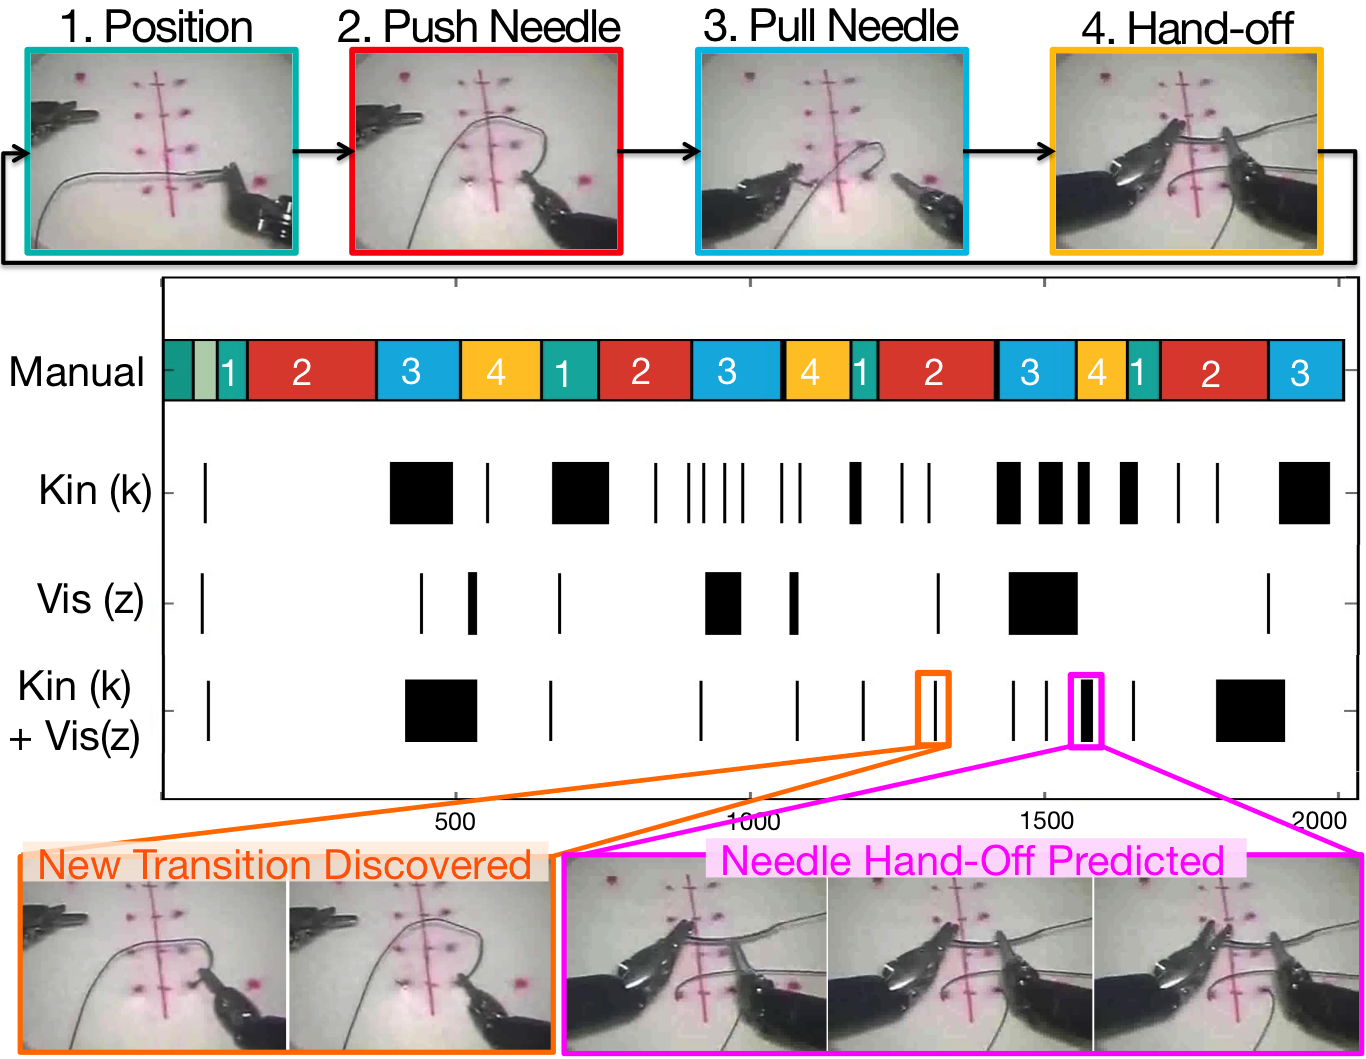
\includegraphics[width=\linewidth]{figures/suturing-v4}
	\caption{The first row shows a manual segmentation of the suturing task in 4 steps: (1) Needle Positioning, (2) Needle Pushing, (3) Pulling Needle, (4) Hand-off. \tsc extracts many of the important transitions without labels and also discovers un-labled transition events.
	\label{fig:suturing}}
\vspace{-15pt}
\end{figure}

% \subsubsection{Synthetic Example}
\vspace{5pt}
\noindent \textbf{1. Synthetic Example: \label{sec:syn}}
We first evaluate \tsc on a synthetic example consisting of 4 linear segments (Figure \figref{toyEx}).
A point robot on a plane moves towards a target in a straight line, once it reaches the target, the target moves to a new location.
This process is repeated four times.
We use the simulation to generate image data and kinematics data.
\figref{toyEx} (b) shows the results of unsupervised segmentation  using only kinematics data ($\binom{x(t)}{y(t)}$). 
When the state is full observed (i.e., we have both x and y positions), we accurately recover 4 segments with kinematics alone.
If we hide one of the states, we see that we can still recover the 4 segments.
In this example, when there is no noise on the kinematics, one dimension alone is enough to learn the segmentation.

Next in \figref{toyEx}, we make this scenario more complex by introducing control noise:
$x(t+1) = x(t)+u(t)+\nu$, where $\nu\, \sim\, \mathcal{N}(0, d_1)$ where $d_1=0.25$
We find that when there is control noise, partial observed kinematics can lead to erroneous segments even in this synthetic example.
We use this example to demonstrate the importance of visual features.
If we add visual features (using SIFT since these are not natural images), we find that we can mitigate the problems caused by noise and partial observability.
Finally, we repeat the above experiment for kinematic sensor noise in the system $\hat{x}(t)= x(t)+\nu$, where $\nu\, \sim\, \mathcal{N}(0, d_2)$ where $d_2 = d_2=0.25$. We note that only the kinematics is corrupted with noise, while the vision sees a straight trajectory. 
%We summarize the results quantitatively in the following table.

%===============================================================
%PR2 figures
% \begin{figure*}[t!]
% 	\centering
% 	\begin{subfigure}[t]{3.4in}
% 	    \centering
%         
\includegraphics[width=0.5\linewidth]{figures/insert}
% % 		\caption{}
% 		\figlabel{lego-pr2}
% 		\vspace{-5pt}
% 	\end{subfigure}
% 	 \hspace{0.1in}
% 	\begin{subfigure}[t]{3.4in}
% 	    \centering
% 		
\includegraphics[width=0.5\linewidth]{figures/insert}
% % 		\caption{}
% 		\figlabel{toyPlane-pr2human}
% 		\vspace{-5pt}
% 	\end{subfigure}
% 	\caption{The figure (a) illustrates the performance of unsupervised segmentation of the 3 Step Lego Assembly Task performed with tele-operated PR2 with two techniques of manual demonstrations. The figure (b) illustrates the comparison of unsupervised segmentation of the Toy Example performed with tele-operated PR2 with two techniques of manual demonstrations.}
% 	\figlabel{pr2_expts}
% % 	\vspace{-10pt}
% \end{figure*}

% \begin{figure*}[t!]
% 	\centering
% 	\begin{subfigure}[t]{3.6in}
% 	    \vspace{0pt}
% 	    \centering
%         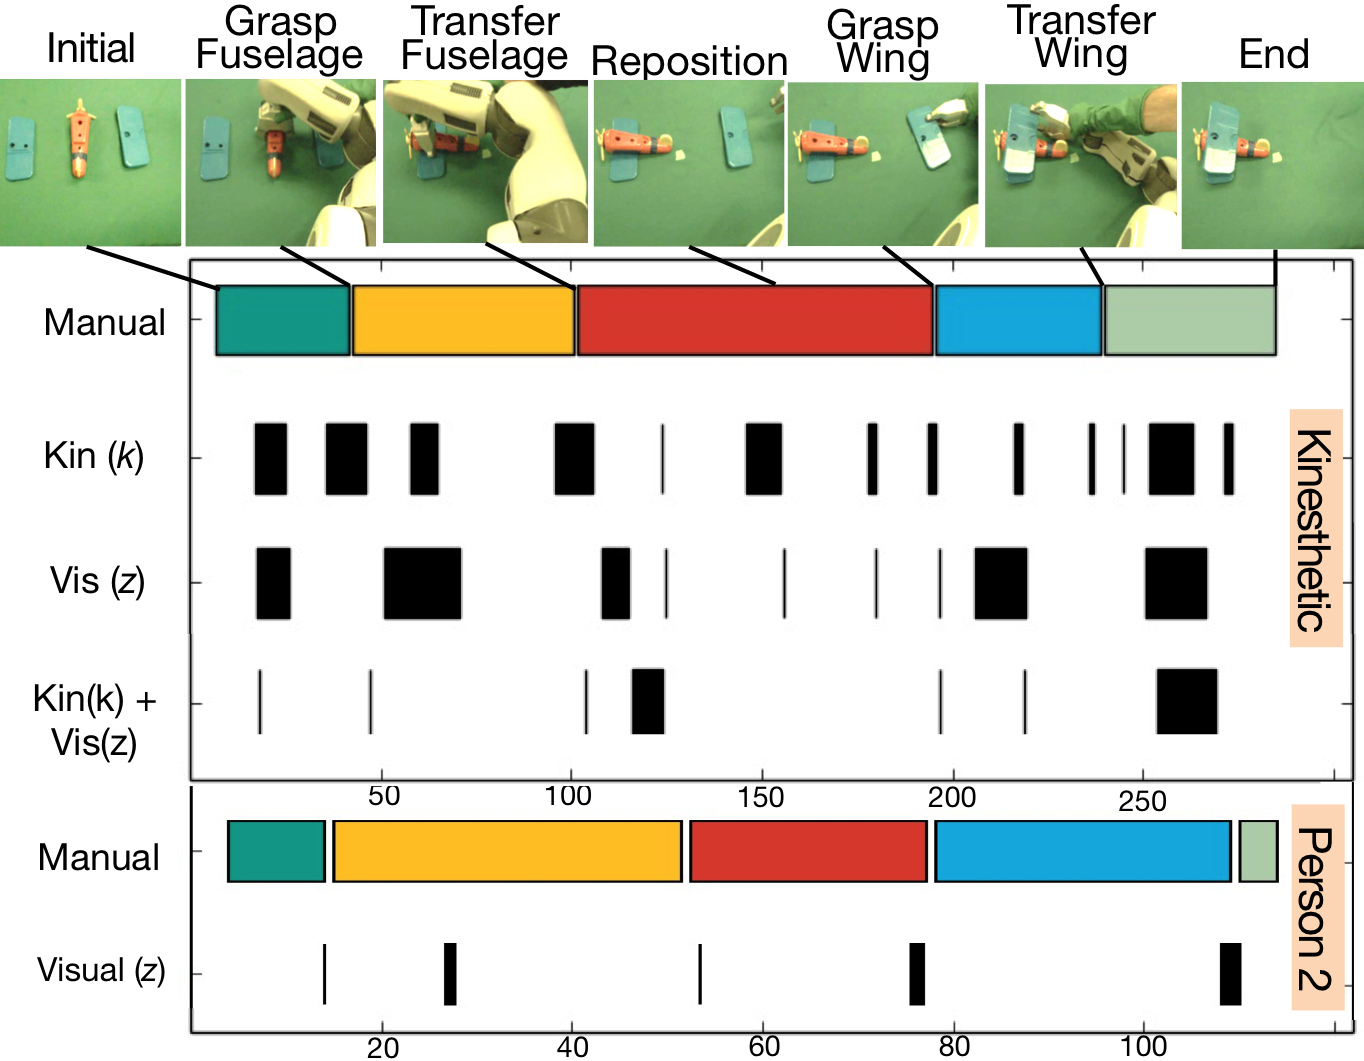
\includegraphics[width=\linewidth]{figures/pr2_plane_assembly}
% % 		\caption{Suturing}
% 		\label{fig:suturing}
% 		\par\vspace{0pt}
% 		\vspace{-10pt}
% 	\end{subfigure}
% 	\begin{subfigure}[t]{2.75in}
%         \vspace{0pt}
%         \centering
%         \resizebox{\linewidth}{!}{% put in textwidth
%             \begin{tabular}{l|l|l|l}
%                 \hline
%                 \multicolumn{1}{c|}{}& \multicolumn{1}{c|}{K} & \multicolumn{1}{c|}{Z} & \multicolumn{1}{c}{K+Z} \\ \hline \hline 
%                 \multicolumn{4}{l}{\cellcolor[HTML]{CBCEFB}Silhouette Score -- Intrinsic Evaluation}  \\
%                 Lego (Robot)    & 0.306$\pm$0.006 & 0.287$\pm$0.051 & \textbf{0.323}$\pm$0.105  \\
%                 \rowcolor[HTML]{E0E0E0}
%                  Plane (Robot)   & 0.481$\pm$0.022 & 0.298$\pm$0.013    & \textbf{0.542}$\pm$0.134 \\
%                 Plane (Person 1) & -- & \textbf{0.202}$\pm$0.020  & -- \\ 
%                 \rowcolor[HTML]{E0E0E0}
%                 Plane (Person 2) & -- & \textbf{0.255}$\pm$0.030  & -- \\ \hline \hline
%                 \multicolumn{4}{l}{\cellcolor[HTML]{FFC72C}NMI Score -- Extrinsic evaluation against manual labels}  \\ 
%                 Lego (Robot)    & 2.97$\pm$0.17\%  & 3.21$\pm$0.35\%  & \textbf{3.04}$\pm$0.25\%  \\
%                 \rowcolor[HTML]{E0E0E0}
%                  Plane (Robot)   & 4.89$\pm$0.6\%   & 4.60$\pm$0.80\%  & \textbf{4.19}$\pm$0.32\%    \\ 
%                 Plane (Person 1) & -- & \textbf{3.88}$\pm$0.93\%  & -- \\ 
%                 \rowcolor[HTML]{E0E0E0}
%                 Plane (Person 2) & -- & \textbf{3.22}$\pm$0.47\%  & -- \\ \hline
%             \end{tabular} 
%         }
%         \caption*{Comparison of \TSC performance on Plane Assembly Task.
%         The segmentation performance is improved with multi-modal data over either modality.
%         % Both tasks show improvements in clustering and prediction accuracy using multi-modal data as compared to either modality. 
%          \textit{Higher} Silhouette Scores and NMI scores are better, respectively. \label{tab:pr2}}
%         \vspace{-15pt}
%         \par\vspace{0pt}
% 	\end{subfigure}
% 	\caption{The figure shows an image sequence from assembly of a toy plane (YCB Dataset). Row 1 is a manual segmentation of the task in 4 steps: Grasp Fuselage, Transfer Fuselage, Grasp Wing, Transfer Fuselage. Rows 2-4 exhibit 
% 	unsupervised the sub-task level segmentation using \tsc. 
% 	\tsc not only learns the segmentations similar to manual labels, but it also discovers unlabeled recurring segments such as arm repositioning. Only vision ($Z$) is used for learning semantically comparable segmentation with human demos.
% % 	Rows 2-4 exhibit the sub-task level segmentation learned by our \del{completely} unsupervised approach using 8 demonstrations. Each row is a sequence of transitions represented by blocks. The width of each block represents the confidence interval conveying the length of transition, with some transitions being near instantaneous while others are gradual.\todo{label figure}
% }
% 	\label{fig:pr2}
% 	\vspace{-15pt}
% \end{figure*}

\iffalse
\begin{table}[bt!]
    \vspace{0pt}
    \centering
    \resizebox{\linewidth}{!}{% put in textwidth
        \begin{tabular}{l|l|l|l}
        \hline
        \multicolumn{1}{c|}{}& \multicolumn{1}{c|}{K} & \multicolumn{1}{c|}{Z} & \multicolumn{1}{c}{K+Z} \\ \hline \hline 
        \multicolumn{4}{l}{\cellcolor[HTML]{CBCEFB}Silhouette Score -- Intrinsic Evaluation}  \\
        Target Noise    & 0.000 $\pm$ 0.000& 0.000 $\pm$ 0.000 & 0.000 $\pm$ 0.000  \\
        \rowcolor[HTML]{E0E0E0}
         Control Noise   & &&\\
        \parbox{2cm}{Kinematics\\ Sensor Noise} & && \\ \hline \hline
        \multicolumn{4}{l}{\cellcolor[HTML]{FFC72C}NMI Score -- Extrinsic evaluation against manual labels}  \\ 
        Target Noise    & && \\
        \rowcolor[HTML]{E0E0E0}
         Control Noise   & &&    \\ 
        \parbox{2cm}{Kinematics\\ Sensor Noise} & &&\\ \hline
        \end{tabular}         
        
    }
    \caption{TABLE II: Quantitative results for the synthetic example}
    \label{tab:toyEx}
    \par\vspace{0pt}
\end{table}
\fi


\vspace{0.25em}
\noindent\textbf{2. Suturing: } 
We apply our method to a subset of JIGSAWS dataset\cite{gao2014jigsaws} consisting of surgical task demonstrations under tele-operation using the da~Vinci surgical system. The dataset was captured from eight surgeons with different levels of skill, performing five repetitions each of suturing and needle passing.
We use 39 demonstrations of a 4 throw suturing task (\figref{suturing}) and we manually annotate these demonstrations for reference.
We apply \tsc to kinematics and vision alone respectively and then the combination.
With combined kinematics and vision, \tsc learns many of the important segments identified by annotation in \cite{gao2014jigsaws}.
After learning the segmentation, we apply it to a representative trajectory and show that we accurately recover 10/15 transitions annotated by our manual labeling.

Upon further investigation of the false positives, we found that they corresponded to crucial actions missed by our labeling.
For example, \tsc discovers that a crucial needle repositioning step where many demonstrators penetrate and push-through the needle in two different motions.
\tsc finds segments that correspond to linear dynamical systems, and applies this criterion consistently.
Human annotators may miss subtle transitions such as quick two-step motions.
%This emphasizes than manual annotation and pre-defined dictionary methods are sensitive to human bias and inconsistency in segmentation criteria.

% applies a more consistent criteria than manual annotation based on domain knowledge.


\begin{table}[t!]
    %\vspace{-10pt}
    \centering
    \resizebox{\linewidth}{!}{% put in textwidth
        \begin{tabular}{ll|l|l|l}
        \\ \hline 
        \multicolumn{2}{c|}{}    & \multicolumn{1}{c|}{K} & \multicolumn{1}{c|}{Z} & \multicolumn{1}{c}{K+Z} \\ \hline \hline
        \multicolumn{5}{l}{\cellcolor[HTML]{CBCEFB}Silhouette Score -- Intrinsic Evaluation} \\
        \cellcolor[HTML]{CBCEFB}                                 & E     & 0.630$\pm$0.014  &  0.576$\pm$0.018  &  0.654$\pm$0.065\\
        \rowcolor[HTML]{E0E0E0}
        \cellcolor[HTML]{CBCEFB}                                 & E+I   & 0.550$\pm$0.014  &  0.548$\pm$0.015  &  0.716$\pm$0.046\\
        \multirow{-3}{*}{\cellcolor[HTML]{CBCEFB}Suturing}       & E+I+N & 0.518$\pm$0.008  &  0.515$\pm$0.021  &  0.733$\pm$0.056\\
        \rowcolor[HTML]{E0E0E0}
        
        \cellcolor[HTML]{FFC72C}                                 & E     & 0.524$\pm$0.004  &  0.609$\pm$0.010  &  0.716$\pm$0.097\\
        \cellcolor[HTML]{FFC72C}                                 & E+I   & 0.521$\pm$0.006  &  0.536$\pm$0.013  &  0.666$\pm$0.067\\
        \rowcolor[HTML]{E0E0E0}
        \multirow{-3}{*}{\cellcolor[HTML]{FFC72C}\parbox{1.2cm}{Needle Passing}} & E+I+N & 0.513$\pm$0.007  &  0.552$\pm$0.011  &  0.557$\pm$0.010\\
        \hline \hline
        
        \multicolumn{5}{l}{\cellcolor[HTML]{FFC72C} NMI Score -- Extrinsic evaluation against manual labels} \\ 
        \cellcolor[HTML]{CBCEFB}                                 & E     &0.516 $\pm$ 0.026 &	0.266 $\pm$ 0.025 & 	0.597 $\pm$ 0.096\\
        \rowcolor[HTML]{E0E0E0}
        \cellcolor[HTML]{CBCEFB}                                 & E+I   & 0.427 $\pm$ 0.053 & 0.166 $\pm$ 0.057   & 0.646 $\pm$ 0.039 \\ 
        \multirow{-3}{*}{\cellcolor[HTML]{CBCEFB}Suturing}       & E+I+N & 0.307 $\pm$ 0.045 &  0.157 $\pm$ 0.022  & 0.625 $\pm $ 0.034  \\ 
        \rowcolor[HTML]{E0E0E0}

           \cellcolor[HTML]{FFC72C}                                 & E     & 0.287 $\pm$ 0.043& 0.222 $\pm$ 0.029& 0.565 $\pm$ 0.037 \\ 
        \cellcolor[HTML]{FFC72C}                                 & E+I   & 0.285 $\pm$ 0.051 & 0.150 $\pm$ 0.048 & 0.471 $\pm$ 0.023  \\ 
        \rowcolor[HTML]{E0E0E0}
        \multirow{-3}{*}{\cellcolor[HTML]{FFC72C}\parbox{1.2cm}{Needle Passing}} & E+I+N & 0.272 $\pm$ 0.035 &  0.186 $\pm$ 0.034  & 0.385 $\pm$ 0.092 \\ \hline
        \end{tabular}
    }
    \caption{Comparison of \TSC performance on Suturing and Needle Passing Tasks. We compare the prediction performance by incrementally adding demonstrations from Experts~(E), Intermediates~(I), and Novices~(N) respectively to the dataset.\label{tab:jigsaws}}
    \par\vspace{0pt}
    \vspace{-15pt}
\end{table}


\vspace{0.25em}
\noindent\textbf{3. Needle Passing: } Next, we applied \tsc to 28 demonstrations of the needle passing task.
These demonstrations were annotated in \cite{gao2014jigsaws}. 
\tabref{jigsaws} lists quantitative results for both needle passing and suturing with both \textsf{ss} and NMI agreement with the human labels.
Demonstrations from the JIGSAWS dataset were annotated with the skill-level of the demonstrators (Expert (E), Intermediate (I), and Novice (I)).
In our surgical datasets, where a mix of skill levels were used, we applied weighted outlier pruning to account for increased outliers amongst novice demonstrators.
We used a weight of $5$ for experts, $2$ for intermediates, and $1$ for novices, and these weights were determined empirically using analysis of task time in the datasets (the max novice time was 5x slower than the expert time).
We present results with weighting on the mixed groups and without weighting on experts only.
We find that in both surgical datasets, kinematics and vision gives improved performance (intrinsically and extrinsically) than either set of features alone.
This emphasizes the benefits of using \tsc as it takes advantage of multimodal trajectory.
Also, we see a strong dependence on the operator's skill level.
The results are very different when applied to just experts compared to all skill levels.
For kinematics and vision alone, the intrinsic metric drops as we add less skilled demonstrations.
However, when we include kinematics and vision we see that the metric increases fur the suturing dataset.
We will investigate this in future work, but we speculate this has to do with sampling error, i.e., adding more data makes the segmentation more accurate.


%In this task, the robot passes a needle through a loop using its right arm, then its left arm to pull the needle through the loop. Then, the robot hands the needle off from the left arm to the right arm. This is repeated four times. 

% \begin{figure}[!t]
% \centering
% 
\includegraphics[width=\linewidth]{figures/insert.png}
% \caption{The figure illustrates the performance of unsupervised segmentation of the 3 Step Lego Assembly Task performed with tele-operated PR2 with two techniques of manual demonstrations.}
%  \label{fig:lego-pr2}
% \vspace{-10pt} 
% \end{figure}

% \begin{figure}[!t]
% \centering
% 
\includegraphics[width=\linewidth]{figures/insert.png}
% \caption{The figure illustrates the comparison of unsupervised segmentation of the Toy Example performed with tele-operated PR2 with two techniques of manual demonstrations.}
%  \label{fig:toyPlane-pr2human}
% \vspace{-10pt} 
% \end{figure}

\begin{figure}[!t]
\centering
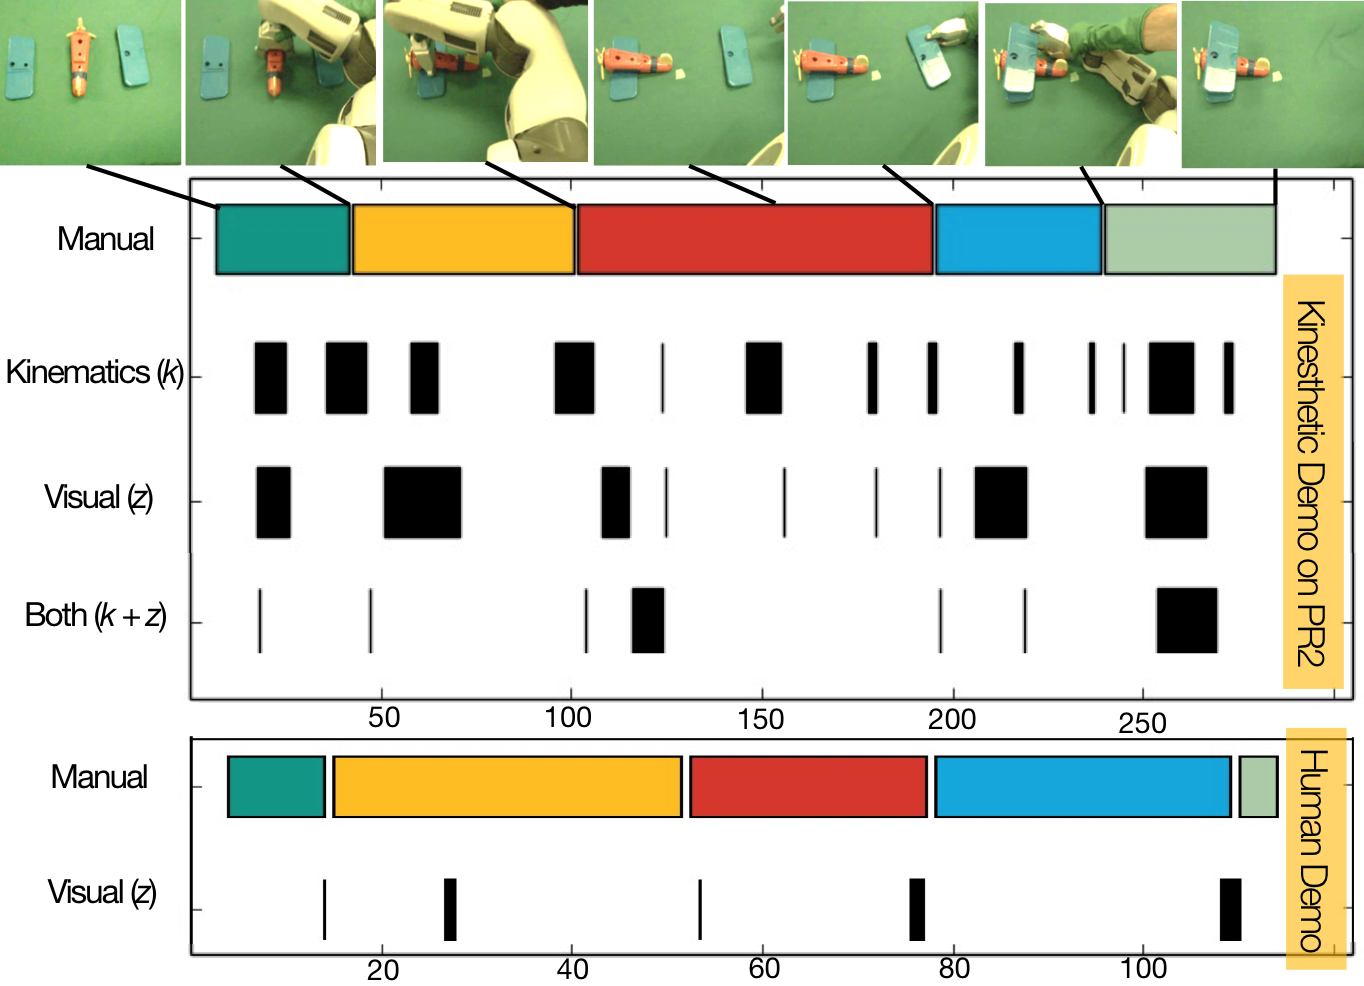
\includegraphics[width=\linewidth]{figures/pr2_plane_assembly-v5}
\caption{We compare \tsc on 12 kinesthetic demonstrations (top) and
8 human demonstrations (bottom).
No kinematics were available for the human demonstrations.
We illustrate the segmentation for an example demonstration of each.
Our manual annotation of the task has 5 steps and \tsc recovers this structure separately for both Kinesthtic demos on PR2 and Human demos with the same visual features. \figlabel{pr2_toyplane}}
\vspace{-20pt}
\end{figure}

\vspace{5pt}
\noindent \textbf{4. PR2: Legos and Toy Plane Assembly: }
In our next experiment, we explore segmenting a multi-step assembly task using (1) large \textit{Lego} blocks and (2) toy \textit{Plane} from the YCB dataset~\cite{calli2015corr}. 
We demonstrate that \tsc applies generally outside of surgical robotics.
We collect 8 kinesthetic demonstrations for each task through kinesthetic demonstrations of the task on the PR2 robot.
\figref{pr2_toyplane} illustrates the segmentation for the plane assembly task.
We find the plane assembly task using kinematics or vision alone results in a large number of segments.
The combination can help remove spurious segments restricting our segments to those tranistions that occur in most of the demonstrations--agreeing in similarity both kinematically and visually.

% \subsubsection{Human Demonstration of Toy Plane Assembly}
\vspace{5pt}
\noindent \textbf{5. Human Demonstration of Toy Plane Assembly: }
We extend the toy plane assembly experiment to collect 8 demonstrations each from two human users. These examples only have videos and no kinematic information. We note that there was a difference between users in the grasping location of fuselage. 
% We used \TSC to learn segmentation for human demonstrations and the results are showed in \figref{toyPlane-pr2human}.
The results of \tsc performance are summarised in Table~\ref{tab:pr2}.
An example of toy plane assembly by both robot and human is qualitatively compared in Figure~\ref{fig:pr2_toyplane}. 
This emphasizes on the benefits of \tsc, namely, that we do not tune the features to any specific robot or task. 
These are general visual features that can apply broadly even when a human is performing demonstrations.
We omit a visualization of the results for the Lego assembly, however, we summarize the results quantitatively in Table \ref{tab:pr2}.

% one example each of the \textit{Lego} and \textit{Plane} assembly task is illustrated in Figures~\ref{fig:lego-pr2} and \ref{fig:pr2_toyplane} respectively.
% The results for clustering evaluation and comparison with a set of manual labels using dynamic time warping distance are tabulated in \tabref{pr2}.


% PR2 TABLE
\begin{table}[!t]
\centering
\resizebox{\linewidth}{!}{% put in textwidth
    \begin{tabular}{l|l|l|l}
        \hline
        \multicolumn{1}{c|}{}& \multicolumn{1}{c|}{K} & \multicolumn{1}{c|}{Z} & \multicolumn{1}{c}{K+Z} \\ \hline \hline 
        \multicolumn{4}{l}{\cellcolor[HTML]{CBCEFB}Silhouette Score -- Intrinsic Evaluation}  \\
        Lego (Robot)    & 0.653$\pm$0.003 & 0.644$\pm$0.026 & 0.662$\pm$0.053 \\
        \rowcolor[HTML]{E0E0E0}
         Plane (Robot)   & 0.741$\pm$0.011 & 0.649$\pm$0.007 & 0.771$\pm$0.067 \\
        Plane (Human 1) & -- & 0.601 $\pm$0.010  & -- \\ 
        \rowcolor[HTML]{E0E0E0}
        Plane (Human 2) & -- & 0.628 $\pm$0.015  & -- \\ \hline \hline
        \multicolumn{4}{l}{\cellcolor[HTML]{FFC72C}NMI Score -- Extrinsic evaluation against manual labels}  \\ 
        Lego (Robot)    & 0.542 $\pm$ 0.058  & 0.712 $\pm$ 0.041  & 0.688 $\pm$ 0.037  \\
        \rowcolor[HTML]{E0E0E0}
         Plane (Robot)   & 0.768 $\pm$ 0.015  & 0.726 $\pm$ 0.040  & 0.747 $\pm$ 0.016    \\ 
        Plane (Human 1) & -- & 0.726 $\pm$ 0.071  & -- \\ 
        \rowcolor[HTML]{E0E0E0}
        Plane (Human 2) & -- & 0.806 $\pm$ 0.034  & -- \\ \hline
    \end{tabular} 
    }
\caption{Plane and Lego Assembly Tasks. Both tasks show improvements in clustering and prediction accuracy using multi-modal data as compared to either modality. Further, only vision ($Z$) is available for human demos of the plane assembly task. Comparable segmentation results are obtained using only video input for human demos. \textit{Higher} Silhoutte Scores and NMI scores are better, respectively. \label{tab:pr2}}
\vspace{-15pt}
\end{table}






\end{document}